\section{Paladin Class Weapons}

\subsubsection{Ashbringer}

It is said that the righteousness of a man is determined by his ability to resist temptations and instead seek what is good for others. Legend has it that true righteousness has only ever been known by one man. An ancient king of Dalaran named Uther. They called him the light-bringer for his righteous acts. Uther reigned from a young boy after his father was killed in battle. He spent his life focused on maintaining peace from attacks from alternate realms and dimensions. It is believed that he was so charismatic that under his reign there was a one rule government. At the end of his life, he was blessed with the opportunity to ascend to a higher plane of existence due to his righteous acts. Upon doing so, he imbued his weapon, Ashbringer, with all of his physical abilities as he shed his body of his soul. It is said that he did this in the catacombs of Ironforge, the great capitol city that they ruled from in these times. The City is said to have been destroyed following the days of his reign when the world broke out into an age changing war. After centuries, all but remains of Ashbringer is but a legend.

\begin{center}
	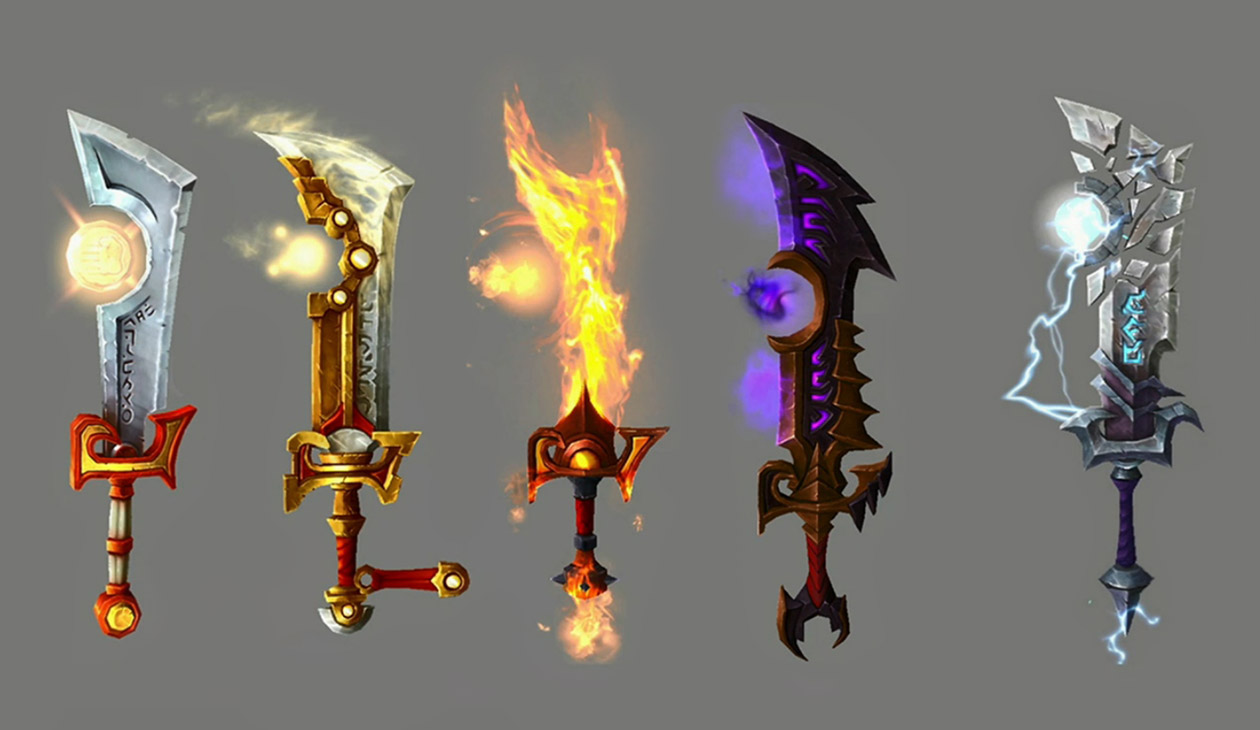
\includegraphics[width=\linewidth]{img/weapons/wowl-ashbringer.jpg}
\end{center}

\subsubsection{Potential}

The Ashbringer weapon wants to be wielded by a righteous character. 

\begin{commentbox}{Ashbringer\footnote{Some information taken from https://www.dndbeyond.com/magic-items/351998-the-ashbringer}\footnote{Weapon (greatsword), artifact (requires attunement by a paladin)}}	
	You gain a +3 bonus to attack and damage rolls made with this magic weapon. When you hit an enemy you will deal 1d6 fire damage and 1d6 radiant damage. The damage will change to d10's if the target is a fiend or an undead.
	
	When you take damage while wielding the Ashbringer, you can heal one target within 50 yards for a single roll of the dice closes to the wielders level (round up).
	
	While a Paladin wields The Ashbringer in combat it will look like the Paladin is burning with a holy flame. Any fiend or undead that attacks the wielder will take 1d6 fire damage and 1d6 radiant damage. When the wielder rolls a 20 against a fiends or an undead the wielder must a d100 roll. If the roll is less than half the wielders lvl then the fiend or undead will burn in holy flame and turn to ash immediately.
	
	If a Paladin of an evil alignment tries to attune to The Ashbringer they have to make a d20 roll. At a 18 or below The Ashbringer will reject you and deal 3d10 fire damage and 2d10 radiant damage. At a 19 or 20 you over power the will of the weapon and make it yours.
	
	With a successful roll to overcome the will of The Ashbringer while having an evil alignment will make The Ashbringers appearance will start to dull and become darker until it becomes fully corrupt. It will regain its former glory when its attuned to a paladin of a non evil alignment.
	
	Proficiency with a greatsword allows you to add your proficiency bonus to the attack roll for any attack you make with it.
	
	If the wielder of Ashbringer dies (by failing three death saves) then the life essence of the blade can leave the weapon and resurrect the player to full. The weapon after this point becomes useless.
\end{commentbox}

\subsubsection{Finding Ashbringer}

Ashbringer is located in an underground vault within the city of Ironforge. Ironforge is located within the Pluvian Forest and has been hidden with time. Ironforge can only be spotted when winter. The snow covering the entrance is slightly melted from the super-heated thermal activities under the cities. The city is mainly collapsed but can be traversed if found. The main gate to the city is closed, but from an avalanche of rocks, part of it is accessible on one side. The Pluvian Forest contains a section stuck in time during an eternal winter, within this winter is where Ironforge is located. From the outside (space-view) this region appears normal, however upon a creature entering this large region, they are transported into a past time when it is winter. 

\begin{center}
	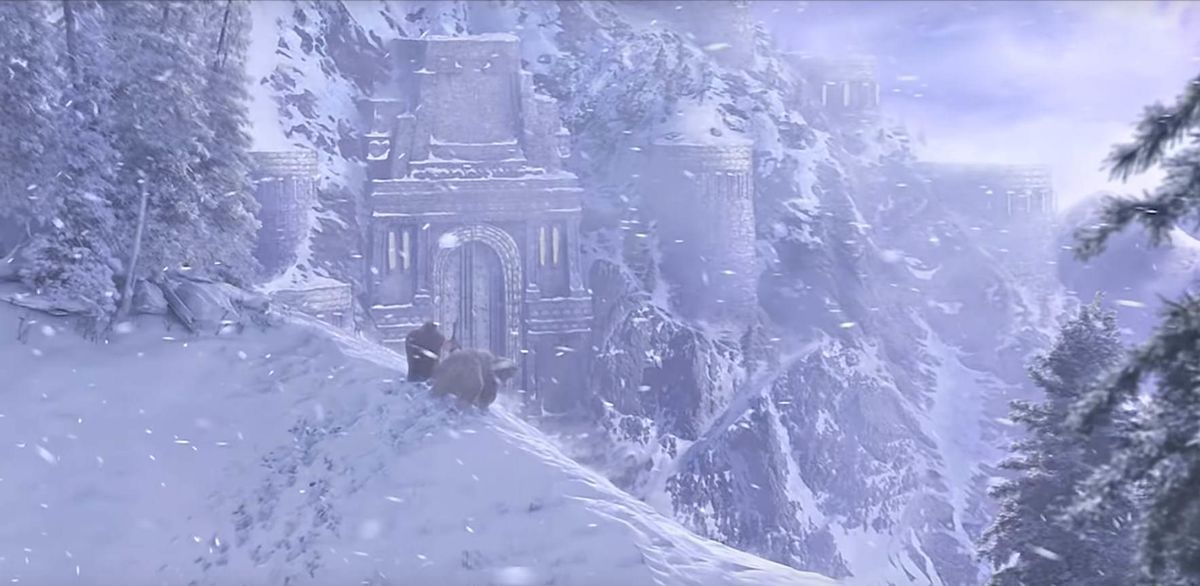
\includegraphics[width=\linewidth]{img/WoW/1200px-Ironforge_-_Classic_cinematic.jpg}
\end{center}

When entering Ironforge, the air is warm and a significant amount of steam is present rising from the thermal ducts throughout the city. The ducts in this state are full of lava that have broken through the lower gates of the vents. Within the center of the city is the kings chamber, where passage to the lower vaults is. Ashbringer is located in the depths of the vault. The vault is a series of large/high paths overlooking magma and lava pits that bubble and steam continually. The area is extremely warm. When approaching Ashbringer, the party will encounter the Firelord Ragnaros. Ragnaros will stop fighting if someone can successfully wield The Ashbringer weapon but will otherwise attack the party and chase them out of the vault.

\begin{center}
	
\includegraphics[width=0.515\linewidth]{img/WoW/ragnaros-1920x1200-heroes-of-the-storm-5781.jpg} 	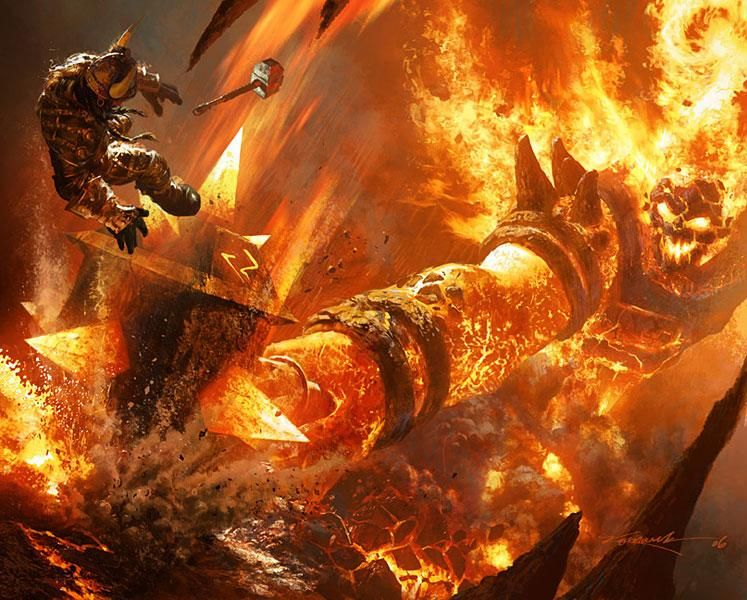
\includegraphics[width=0.45\linewidth]{img/WoW/b9e0808495e9cf3dcbbecedf3e4d5e32.jpg}
\end{center}

\begin{monsterbox}{Ragnaros The Firelord}
	This character design is taken from https://www.dndbeyond.com/monsters/82907-ragnaros
	\begin{hangingpar}
		\textit{Gargantuan Fiend, neutral evil}
	\end{hangingpar}
	\dndline%
	\basics[%
	armorclass = 23,
	hitpoints  = 533,
	speed      = 50 ft
	]
	\dndline%
	\stats[
	STR = \stat{30}, % This stat command will autocomplete the modifier for you
	DEX = \stat{20},
	CON = \stat{30},
	INT = \stat{30},
	WIS = \stat{24},
	CHA = \stat{30}
	]
	\dndline%
	\details[%
	% If you want to use commas in these sections, enclose the
	% description in braces.
	% I'm so sorry.
	languages = {All, Telepathy 5 miles},
	challenge = 30
	]
	\dndline%
	saving throws = STR +19, DEX +14, CON +19, INT +19, WIS +16, CHA +19
		
	skills = Deception +28, Insight +25, Perception +16, Persuasion +28
		
	damage resistance = Cold
	 
	damage immunities = Fire, Lightning, Poison; Bludgeoning, Piercing, and Slashing from Nonmagical Attacks that aren't Silvered
		
	condition immunities = Exhaustion, Petrified, Poisoned	
	
	Senses = Truesight 120 ft., Passive Perception 20
	
	\dndline%
	\begin{monsteraction}[Fear aura]
		Any creature hostile to Ragnaros that starts its turn within 20 feet of Ragnaros must make a DC 24 Wisdom saving throw, unless Ragnaros is incapacitated. On a failed save, the creature is frightened until the start of its next turn. If a creature's saving throw is successful, the creature is immune to Ragnaros's Fear Aura for the next 24 hours.
	\end{monsteraction}	
	\begin{monsteraction}[Death Throes]
		When Ragnaros dies, it explodes, and each creature within 30 feet of it must make a DC 20 Dexterity saving throw, taking 105 (30d6) fire damage on a failed save, or half as much damage on a successful one. The explosion ignites flammable objects in that area that aren't being worn or carried, and it destroys the balor's weapons.
	\end{monsteraction}	
	\begin{monsteraction}[Fire Aura]
		At the start of each of Ragnaros's turns, each creature within 5 feet of it takes 10 (3d6) fire damage, and flammable objects in the aura that aren't being worn or carried ignite. A creature that touches Ragnaros or hits it with a melee attack while within 5 feet of it takes 10 (3d6) fire damage.
	\end{monsteraction}	
	\begin{monsteraction}[Magic Weapon]
		The pit fiend's weapon attacks are magical.
	\end{monsteraction}	
	\begin{monsteraction}[Innate Spellcasting]
		The pit fiend's spellcasting ability is Charisma (spell save DC 23). Ragnaros can innately cast the following spells, requiring no material components:
		
		\begin{itemize}
			\item At will: detect magic, fireball, burning hands, charm person
		
			\item 3/day each: hold monster, wall of fire, 
		
			\item 2/day each: incendiary cloud, delayed blast fireball, dominate person
		
			\item 1/day each: meteor swarm, storm of vengeance 
		\end{itemize}
	\end{monsteraction}	
	\monstersection{Actions}
	\begin{monsteraction}[Multiattack]
		Ragnaros makes five attacks: one with its bite, two with its claw, one with its mace, and one with its lightning whip.
	\end{monsteraction}	
	\begin{monsteraction}[Bite]
		Melee Weapon Attack: +14 to hit, reach 5 ft., one target. Hit: 22 (4d6 + 8) piercing damage plus 14 (4d6) fire damage.  The target must succeed on a DC 21 Constitution saving throw or become poisoned. While poisoned in this way, the target can't regain hit points, and it takes 21 (6d6) poison damage at the start of each of its turns. The poisoned target can repeat the saving throw at the end of each of its turns, ending the effect on itself on a success.
	\end{monsteraction}	
	\begin{monsteraction}[Claw]
		Melee Weapon Attack: +19 to hit, reach 10 ft., one target. Hit: 19 (2d8 + 10) slashing damage.
	\end{monsteraction}	
	\begin{monsteraction}[Mace]
		Melee Weapon Attack: +19 to hit, reach 10 ft., one target. Hit: 17 (2d6 + 10) bludgeoning damage plus 35 (10d6) fire damage.
	\end{monsteraction}	
	\begin{monsteraction}[Lightning Whip]
		Melee Weapon Attack: +19 to hit, reach 30 ft., one target. Hit: 17 (2d6 + 10) slashing damage plus 35 (10d6) lightning damage, and the target must succeed on a DC 20 Strength saving throw or be pulled up to 25 feet toward Ragnaros
	\end{monsteraction}	
	\begin{monsteraction}[Polymorph]
		Ragnaros can take the form of a gargantuan molten titan (his actual form) or of any devil or demon and uses the stats of that form, if he is killed in one of these forms he begins regenerating in his lair and cant take form for a time, he is only killed if he dies in his actual form
	\end{monsteraction}	
	\begin{monsteraction}[Teleport]
		Ragnaros magically teleports, along with any equipment he is wearing or carrying, up to 120 feet to an unoccupied space it can see.
	\end{monsteraction}	
	\monstersection{Legendary Actions}
	Ragnaros can take 3 legendary actions, choosing from the options below. Only one legendary action option can be used at a time and only at the end of another creature's turn. Ragnaros regains spent legendary actions at the start of its turn.
	\begin{monsteraction}[Detect]
		Ragnaros makes a Wisdom (Perception) check.
	\end{monsteraction}
	\begin{monsteraction}[Lightning Whip]
		Ragnaros makes a Lightning whip attack.
	\end{monsteraction}
	\begin{monsteraction}[Use Spell (costs 2 actions]
		Ragnaros Casts one of his spells. expending a spell slot as normal
	\end{monsteraction}
	\monstersection{Description/Information}
	Ragnaros is actually a demon and devil fused into 1 being and is incredibly powerful, rivalling Asmodeus himself. When he wishes he can take the form of a gargantuan mountain of molten rock and fire or he can take the form of any demon or devil, There is a place on the material plane known as the Elemental Valley known for it containing portals to all 4 of the elemental planes, deep under this valley is where Ragnaros is locked for eternity,
\end{monsterbox}

